\subsubsection{Tạo tăng cường truy xuất (Retrieval Augmented Generation)}

Mô hình ngôn ngữ lớn
có thể đưa ra kết quả không chính xác trong thực tế,
đối mặt với thách thức như hiểu được lập luận pháp lý phức tạp,
đảm bảo tính minh bạch và tránh các phản hồi gây hiểu nhầm.
Làm thế nào để mô hình ngôn ngữ lớn có thể trả lời các câu hỏi pháp luật một cách chính xác?
Retrieval Augmented Generation (RAG)
là một kỹ thuật
được thiết kế
để khắc phục hiện tượng ảo giác
của LLM
bằng cách cung cấp thêm nguồn tri thức bên ngoài
trước khi sinh ra câu trả lời.
Trong phạm vi đồ án này,
em sử dụng
% Agentic
RAG
để tăng cường khả năng truy xuất tri thức từ các văn bản pháp luật,
giúp mô hình ngôn ngữ lớn đưa ra câu trả lời chính xác hơn,
có căn cứ pháp lý rõ ràng
và giảm thiểu hiện tượng ảo giác so với mô hình LLM truyền thống.
Thay vì “đoán”, LLM sẽ dựa vào dữ liệu thật
từ đó cung cấp nguồn dẫn chứng rõ ràng cho người dùng.
% \end{block}

% Phương pháp này thực hiện bằng cách truy xuất thông tin liên quan từ kho tài liệu (tri thức)
% và sử dụng chúng cho quá trình sinh câu trả lời dựa trên LLMs.

% Ở góc nhìn triển khai hệ thống, các kiến trúc RAG hiện đại thường được mô tả như một pipeline gồm 3 giai đoạn chính:

% Lập chỉ mục (indexing): Chuẩn hóa dữ liệu và xây dựng chỉ mục truy xuất.
% Truy xuất (retrieval): Tìm các đoạn văn bản liên quan nhất với truy vấn.
% Tạo sinh (generation): LLM sử dụng các đoạn truy xuất làm ngữ cảnh để tổng hợp và tạo câu trả lời.

\begin{figure}[H]
\centering
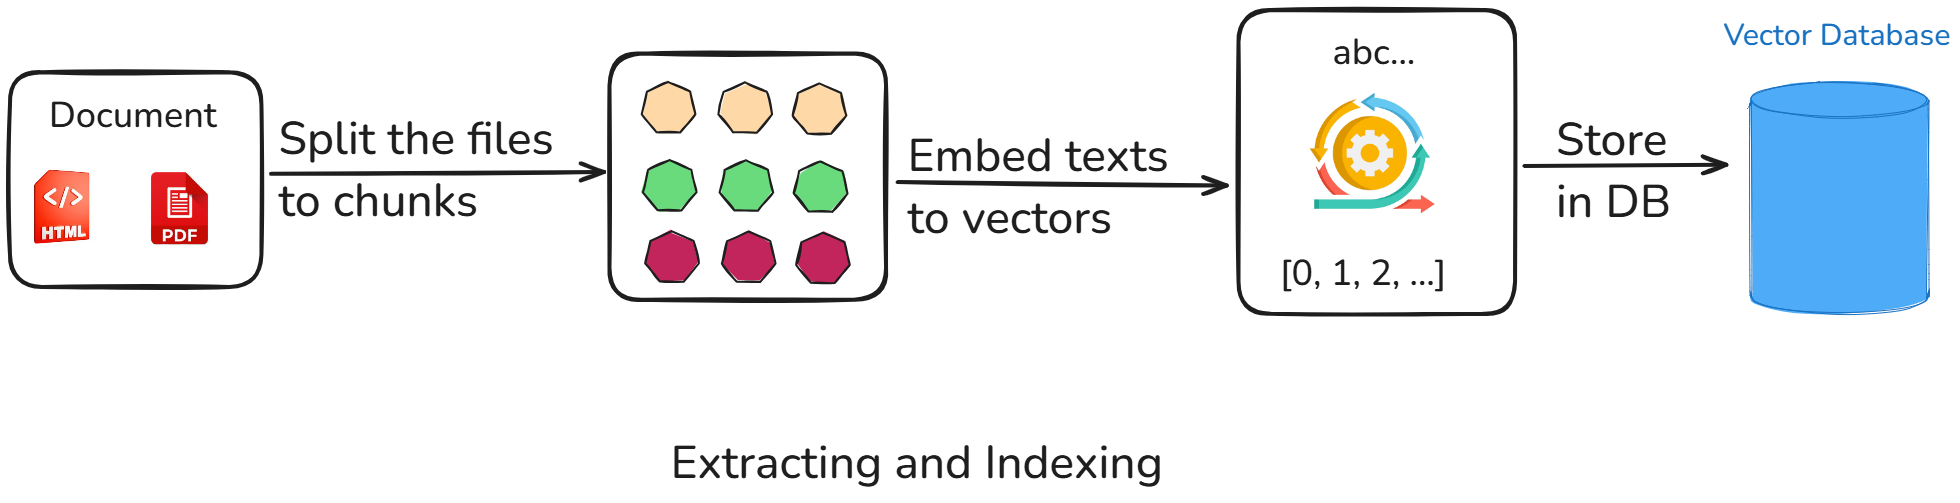
\includegraphics[scale = 0.20]{pictures/rag-1.excalidraw.png}
\caption{Sơ đồ RAG cơ bản (Extracting and Indexing)}
\end{figure}

% TODO RAG rẻ hơn tinh chỉnh

% TODO Các cách chucking

Các bước cốt lõi để xây dựng một hệ thống RAG:

\begin{itemize}

\item Toàn bộ dữ liệu tri thức (tài liệu, văn bản luật, \dots) được chia nhỏ thành các đoạn (chunks).

\item Sử dụng các mô hình nhúng (embedding models) để chuyển đổi các đoạn văn bản này thành các biểu diễn vector.

\item Lưu trữ các vector vào vector database để tối ưu hóa việc tìm kiếm không gian nhiều chiều.

\item Hệ thống nhận yêu cầu từ người dùng dưới dạng ngôn ngữ tự nhiên.

\item Câu truy vấn của người dùng cũng được mã hóa thành vector.
\item Cơ chế truy xuất sẽ quét toàn bộ vector database để đo lường độ tương đồng ngữ nghĩa nhằm trích xuất ra các đoạn tài liệu liên quan nhất.

\item Các đoạn văn bản liên quan vừa được truy xuất sẽ được ghép nối với câu truy vấn ban đầu của người dùng.

\item Câu prompt đã được làm giàu ngữ cảnh sẽ được đưa vào LLM
\item LLM sử dụng ngữ cảnh được cung cấp để sinh ra câu trả lời mạch lạc và có độ chính xác cao đối với nguồn dữ liệu.

\end{itemize}

Việc áp dụng kiến trúc RAG không chỉ giúp giảm đáng kể chi phí huấn luyện và bảo trì mô hình mà còn hạn chế hiện tượng tạo ra thông tin ảo giác thông qua việc dựa trên các tài liệu được truy xuất từ nguồn dữ liệu đáng tin cậy. Điều này giúp nâng cao độ chính xác, khả năng mở rộng và tính cập nhật của hệ thống.

\begin{figure}[H]
\centering
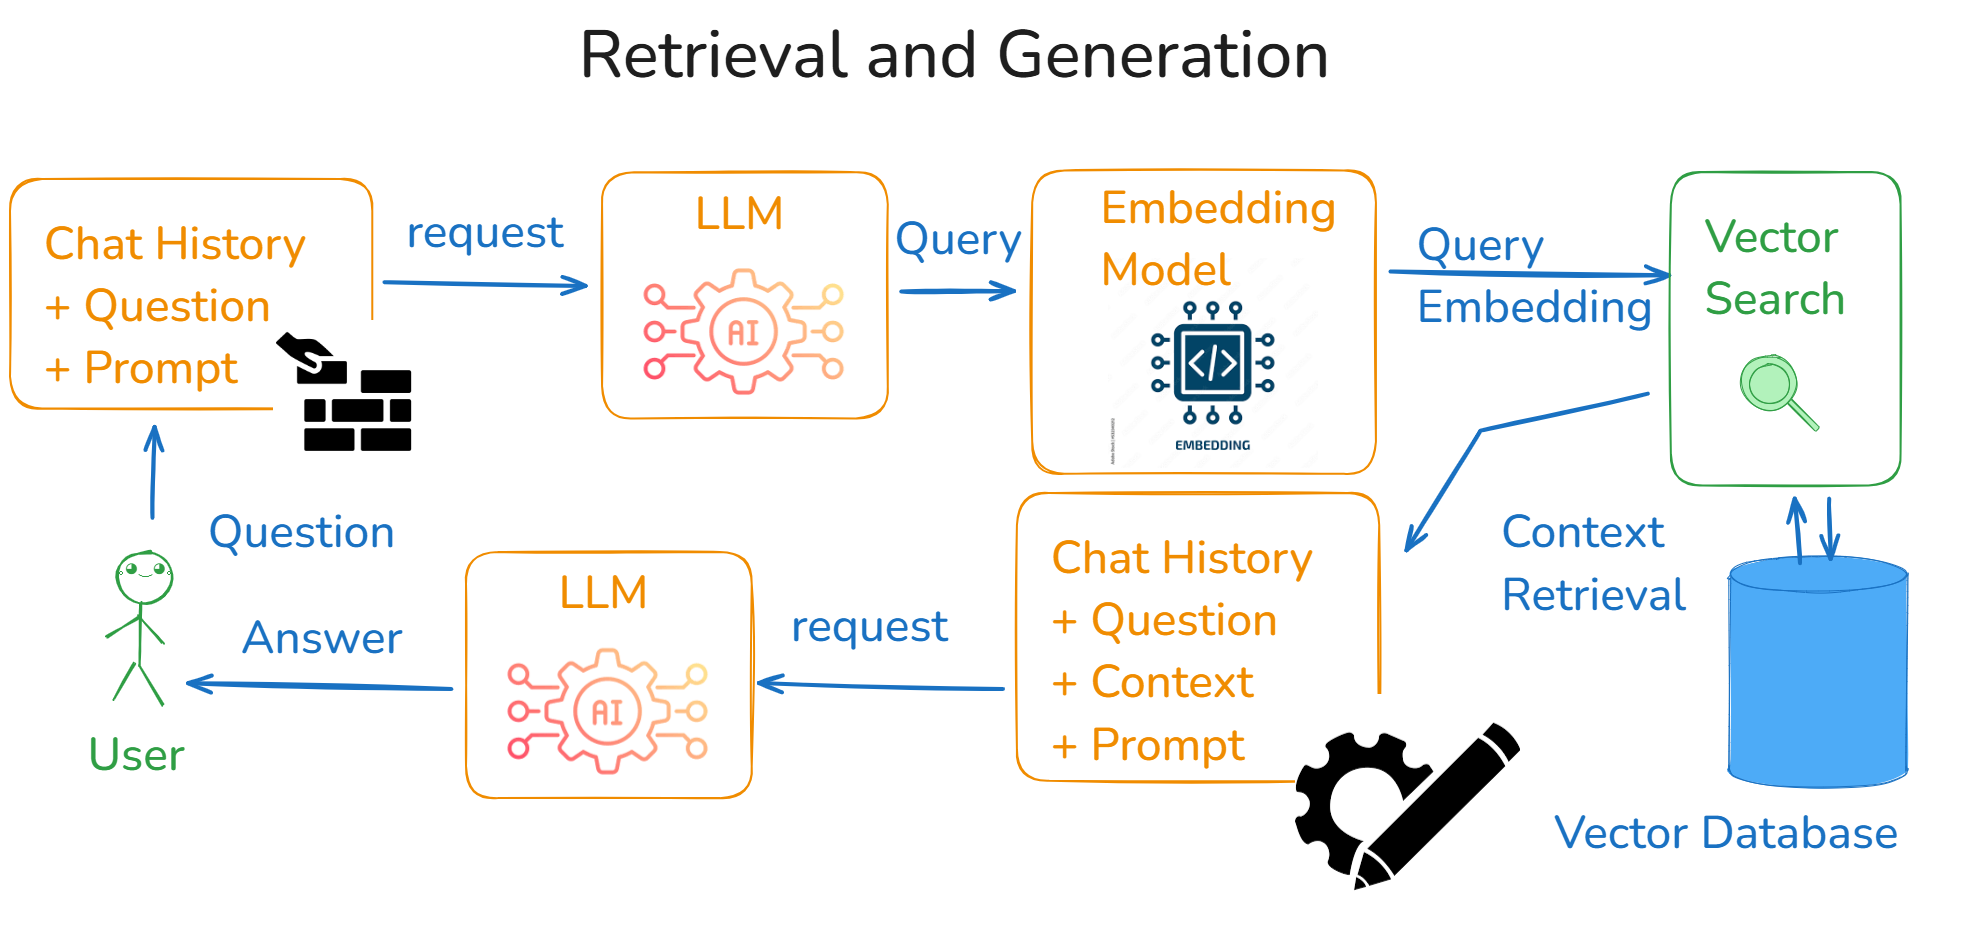
\includegraphics[scale = 0.21]{pictures/rag-2.excalidraw.png}
\caption{Sơ đồ RAG cơ bản (Retrieval and Generation)}
\end{figure}

% Hệ sinh thái LangChain trong phát triển ứng dụng AI:

% \begin{itemize}

% \item LangChain cung cấp các khối xây dựng cơ bản như lời nhắc, mô hình, bộ nhớ và bộ truy xuất để kết hợp thành các quy trình tuyến tính.

% \item LangGraph mô hình hóa các ứng dụng AI dưới dạng đồ thị cho phép các tác nhân lặp lại, phân nhánh, đánh giá kết quả và duy trì trạng thái trung tâm, làm cho nó trở nên lý tưởng cho các hệ thống đa tác nhân.

% \item LangSmith và Langfuse cung cấp khả năng theo dõi và phân tích để gỡ lỗi, theo dõi việc sử dụng token và đánh giá hiệu suất.

% \end{itemize}

% TODO: Sử dụng LangSmith trong dự án
% TODO: Sử dụng Langfuse trong dự án
